\subsection{Revis\~ao sistem\'atica da literatura} \label{subsec:revisão}

As séries temporais aparecem em vários campos do conhecimento, tais como Economia (preços de estoque diários, taxa de desemprego mensal, produção industrial), Medicina (eletrocardiograma, eletroencefalograma), Epidemiologia (número mensal de novos casos de meningite), Meteorologia (chuvas, temperatura diária, velocidade do vento), etc. Ao longo dos anos tem usado ferramentas computacionais para tornar esta previsão mais eficiente, com aprendizagem de máquinas e algumas características que podem ser aplicadas em linguagem computacional através da linguagem \textit{python e R}, as melhores linguagens para trabalhar com séries temporais hoje em dia.

Para entender melhor este conceito de série temporal, suponhamos que um maratonista que esteja correndo há vários anos e uma pessoa sedentária se submeta a uma corrida de, no máximo, $5$ km, ambos corram ao mesmo tempo para que tenham um monitor de frequência cardíaca para que possa ser monitorado por um médico se você pegar os dados desde o início e compará-los com o final da corrida, o maratonista terá uma série mais estacionária porque ele tem o hábito de correr regularmente enquanto a pessoa sedentária terá uma série não estacionária como mostrado na Figura \ref{fig:series}.


\begin{figure}[H]
	\centering
	\caption{Exemplo de séries temporais}
	\label{fig:series}
	\includegraphics[width=0.9\linewidth]{Revisao/Figuras/séries}
	
	Fonte: \cite{brandão_2020}
\end{figure}


Na figura \ref{fig:series} observa-se que o eixo $x$ representa os dados observados e $t$ para o tempo percorrido.
Além disso, as séries temporais são processos estocásticos por leis probabilísticas, o que significa que há a possibilidade de ser pensado como um conjunto de todas as trajetórias possíveis na Figura \ref{fig:series} é capaz de ser observado para uma variável alvo. Por exemplo, se você lançar um dado qualquer valor inteiro entre 1 e 6, mas apenas um número ocorrerá. Da mesma forma, em séries temporais existem infinitas possibilidades, entre elas apenas uma de acordo com as características que atenderam a esse período e que de fato ocorrerão.

\begin{figure}[H]
	\centering
	\caption{Processo estocástico}
	\label{fig:serie}
	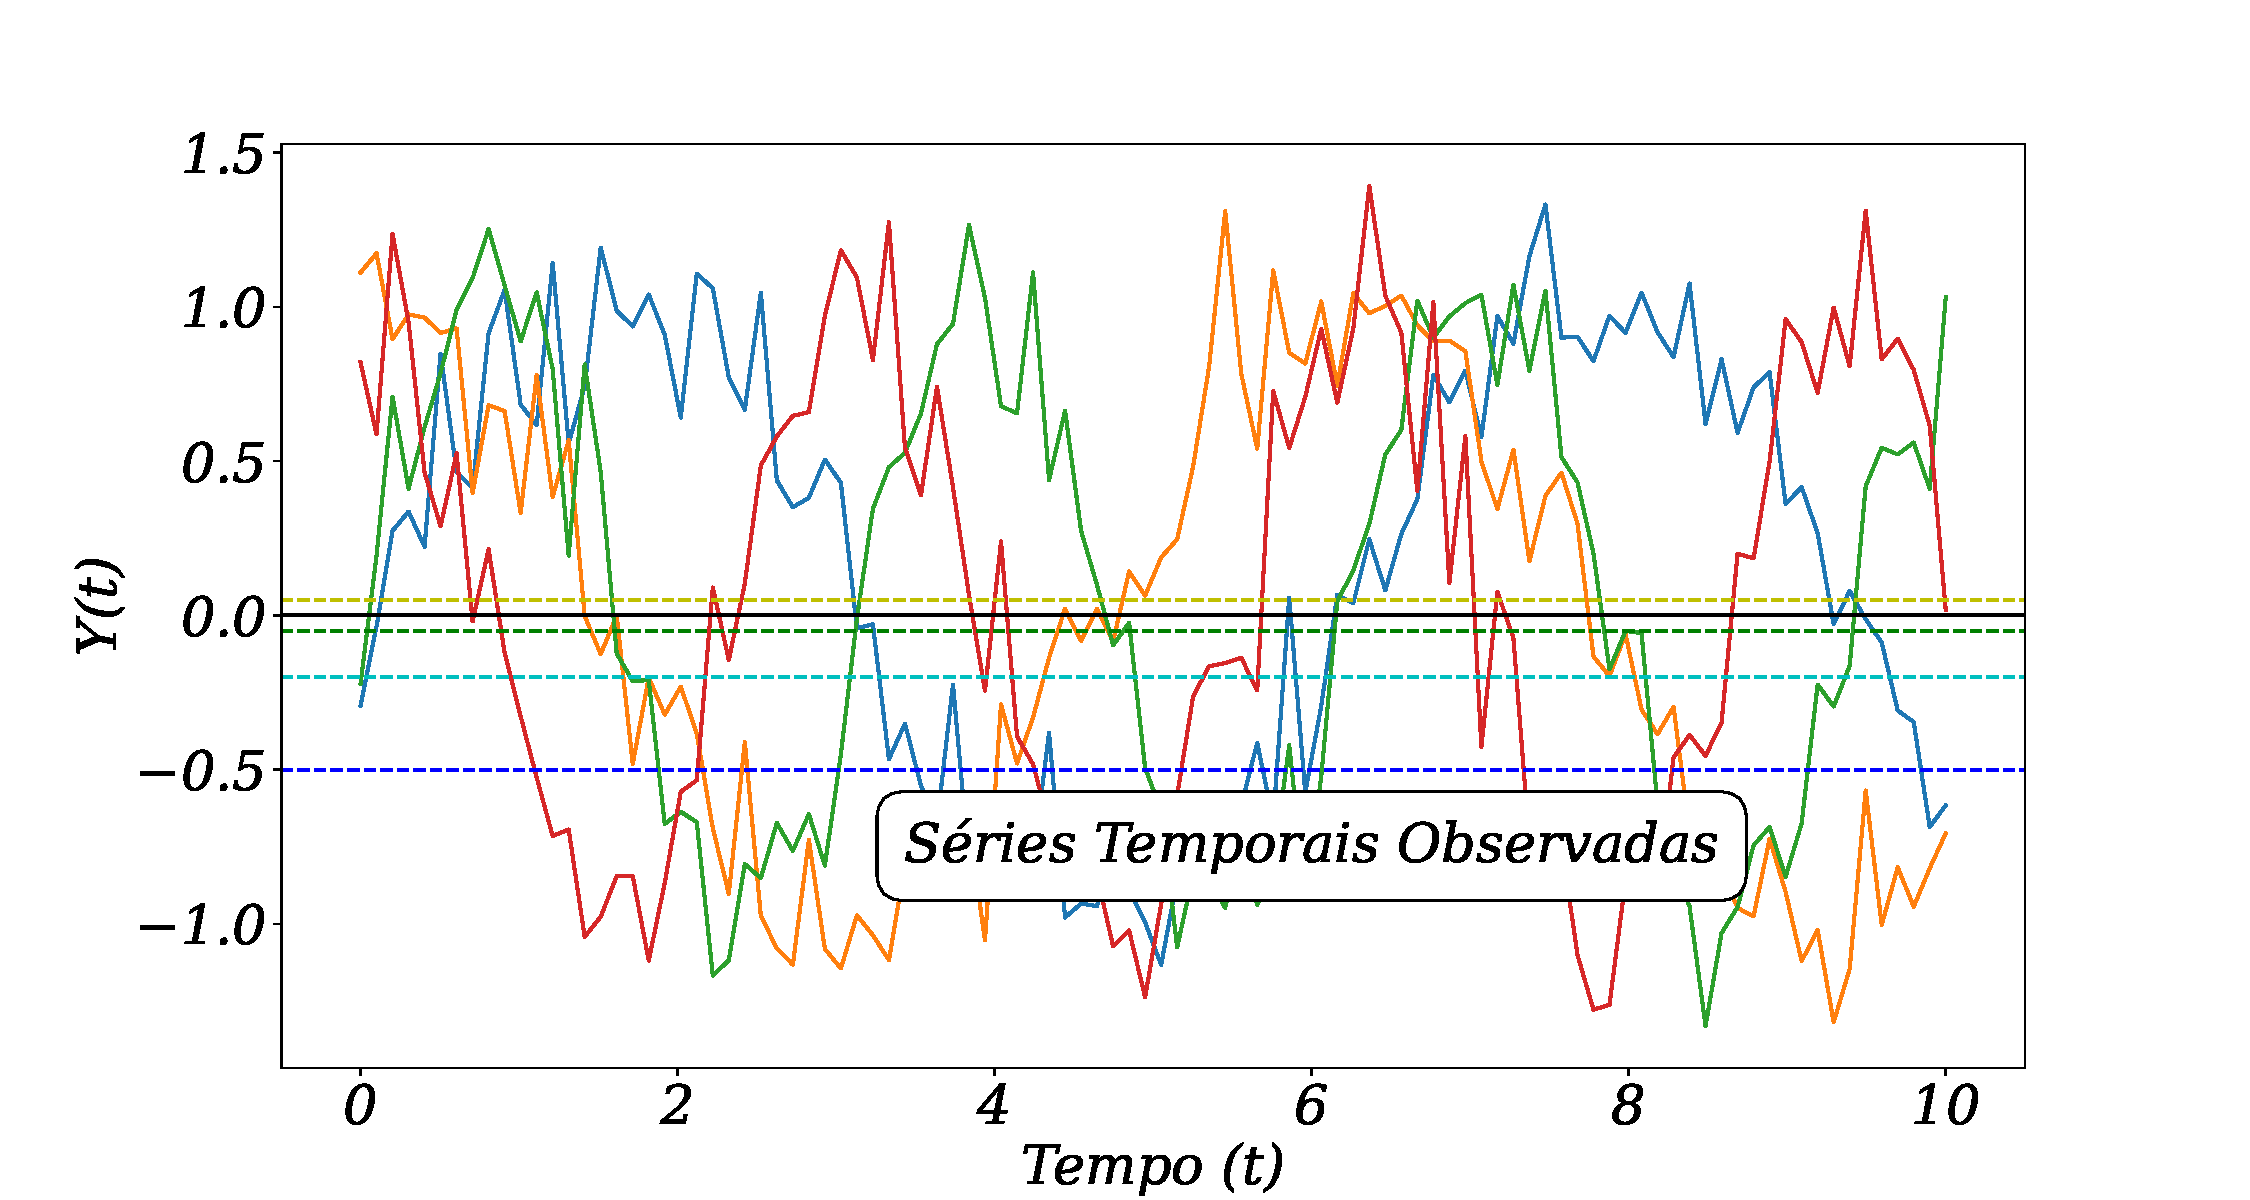
\includegraphics[width=1\linewidth]{Revisao/Figuras/serie}
	
	Fonte: \cite{pinheiro_2022}
\end{figure}

Com $Y(t)$ os dados fictícios e $Tempo \ (t)$ a linha do tempo da Figura \ref{fig:series}.

De repente é pensado como um conjunto de todas as trajetórias possíveis que poderiam ser para observar uma variável.


Esta revisão sistemática da literatura, com o tema abordado até agora é sobre séries temporais, considerando o contexto aqui exposto este tema pode ser de grande relevância em diversas áreas, como mostrado na Figura \ref{fig:areas}. Realizando esta análise de séries temporais nos últimos 6 anos para poder observar as melhores realizações neste tema abordado aqui um curto período, mas tendo o tempo não muito a favor, então teve a opção de deixar este tempo específico para buscar artigos.

O objetivo desta revisão é analisar uma literatura menor, mas muito relevante. Como a própria série temporal procura analisar e modelar a dependência e considerando a ordem apresentada nas bases, por exemplo, os maiores autores e o ano de atividade que mais publicaram nos países que têm o maior número de publicações na apresentação das palavras-chave que serão mostradas, o objetivo é rever cada coisa que pode ser usada em uma aplicação de aprendizagem de máquina.

Em todos os artigos observados que tem uma contribuição científica neste trabalho é a análise do conceito de série temporal com o melhor uso das palavras-chave mesmo não tendo uma grande relação na aprendizagem de máquinas podem ser usados estes artigos como base para outros pesquisadores, aqui algumas análises muito simples para alguns leitores. Entretanto, é um ponto de partida para muitos que não conhecem o conceito de séries cronológicas ou revisão sistemática da literatura.
